\subsection{Exemple 1 : Ordonancement des tâches}
\label{subsec:exemple_1}

Pour mieux comprendre le fonctionnement de l'ordonanceur et des tâches, un exemple de scénario
d'utilisation est donné ci-dessous.\\

- En premier lieu, les tâches A, B, C, D et E sont ajoutées dans une zone mémoire alloué au moment de
l'initilisation de l'ordonanceur et leur addresse mémoire respective sont placées dans le tableau
\texttt{task}. Puisqu'elles sont toutes en cours d'exécution, les booléens correspondants à leur index
dans le tableau \texttt{running} sont à \texttt{true}. (L'addresse mémoire de chaque tâche sera noté
"\&X" où X est le nom de la tâche.) 

\begin{figure}[h]
    \centering
    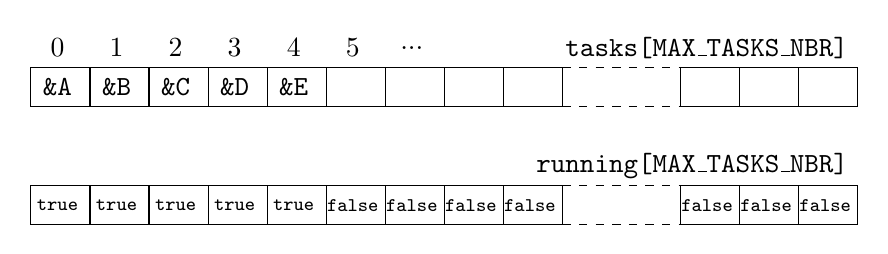
\begin{tikzpicture}[yscale=1, xscale=1.5]
        % \draw[help lines] (-5,-1) grid (5, 2);

        \draw node at (-4.775, 1.25) {0};
        \draw node at (-4.275, 1.25) {1};
        \draw node at (-3.775, 1.25) {2};
        \draw node at (-3.275, 1.25) {3};
        \draw node at (-2.775, 1.25) {4};
        \draw node at (-2.275, 1.25) {5};
        \draw node at (-1.775, 1.25) {...};

        \draw node[anchor=east] at (2, 1.25) {\texttt{tasks[MAX\_TASKS\_NBR]}};
        \draw[step=0.5] (-5.0, 0.5) grid (-0.5, 1);
        \draw[step=0.5] (+0.5, 0.5) grid (+2.0, 1);
        \draw[dashed] (-0.5, 1.0) -- (+0.5, 1.0);
        \draw[dashed] (-0.5, 0.5) -- (+0.5, 0.5);

        \draw node at (-4.775, 0.75) {\texttt{\&A}};
        \draw node at (-4.275, 0.75) {\texttt{\&B}};
        \draw node at (-3.775, 0.75) {\texttt{\&C}};
        \draw node at (-3.275, 0.75) {\texttt{\&D}};
        \draw node at (-2.775, 0.75) {\texttt{\&E}};
        
        \draw[step=0.5] (-5.0, -0.5) grid (-0.5, -1);
        \draw[step=0.5] (+0.5, -0.5) grid (+2.0, -1);
        \draw[dashed] (-0.5, -1.0) -- (+0.5, -1.0);
        \draw[dashed] (-0.5, -0.5) -- (+0.5, -0.5);
        \draw node[anchor=east] at (2, -0.25) {\texttt{running[MAX\_TASKS\_NBR]}};

        \draw node at (-4.775, -0.75) {\scriptsize\texttt{true}};
        \draw node at (-4.275, -0.75) {\scriptsize\texttt{true}};
        \draw node at (-3.775, -0.75) {\scriptsize\texttt{true}};
        \draw node at (-3.275, -0.75) {\scriptsize\texttt{true}};
        \draw node at (-2.775, -0.75) {\scriptsize\texttt{true}};
        \draw node at (-2.275, -0.75) {\scriptsize\texttt{false}};
        \draw node at (-1.775, -0.75) {\scriptsize\texttt{false}};
        \draw node at (-1.275, -0.75) {\scriptsize\texttt{false}};
        \draw node at (-0.775, -0.75) {\scriptsize\texttt{false}};
        \draw node at ( 0.725, -0.75) {\scriptsize\texttt{false}};
        \draw node at ( 1.225, -0.75) {\scriptsize\texttt{false}};
        \draw node at ( 1.725, -0.75) {\scriptsize\texttt{false}};
    \end{tikzpicture}
    \caption{Schéma des tableaux tasks et running de l'ordonanceur (1)}
    \label{fig:async_scheduler_0}
\end{figure}

- Ensuite, la tâche C se termine et se retire de l'ordonanceur. Son booléen correspondant dans
le tableau \texttt{running} est alors à \texttt{false}. Prenons cet exemple pour expliquer
comment les tâches sont exécutées par l'ordonanceur. A chaque fois que la fonction
\texttt{run\_scheduler}\footnoteref{footnote:ref_async_h} est appelée, l'ordonanceur exécute la tâche suivante. Cette dernière
correspond à la première tâche dont le booléen correspondant dans le tableau \texttt{running}
est à \texttt{true} depuis l'index \texttt{current\_idx} jusqu'à ce que l'ensemble des
tâches aient été exécutées. Dans le cas de la figure \ref{fig:async_scheduler_1}, au premier
tour de boucle, la tâche A est exécutée, puis la tâche B, puis la tâche D et enfin la tâche E.
La tâche C n'est pas exécutée car son booléen correspondant dans le tableau \texttt{running}
est à \texttt{false}. \texttt{current\_idx} passe alors respectivement de 0, 1, 3, et 4.
Ensuite, puisque toutes les tâches ont été parcourues une fois, la tâche suivante est la tâche
A. Cela est répété jusqu'à ce que toutes les tâches soient retirées de l'ordonanceur.

\begin{figure}[h]
    \centering
    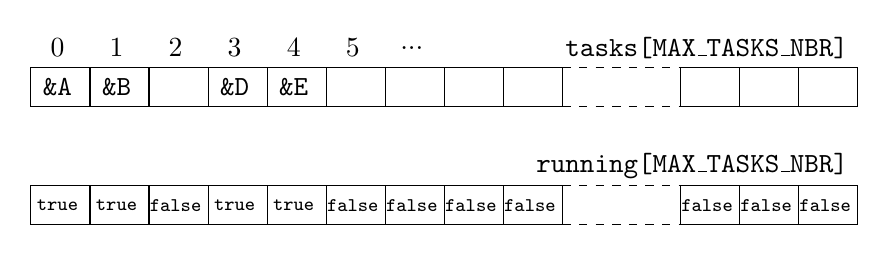
\begin{tikzpicture}[yscale=1, xscale=1.5]
        % \draw[help lines] (-5,-1) grid (5, 2);

        \draw node at (-4.775, 1.25) {0};
        \draw node at (-4.275, 1.25) {1};
        \draw node at (-3.775, 1.25) {2};
        \draw node at (-3.275, 1.25) {3};
        \draw node at (-2.775, 1.25) {4};
        \draw node at (-2.275, 1.25) {5};
        \draw node at (-1.775, 1.25) {...};

        \draw node[anchor=east] at (2, 1.25) {\texttt{tasks[MAX\_TASKS\_NBR]}};
        \draw[step=0.5] (-5.0, 0.5) grid (-0.5, 1);
        \draw[step=0.5] (+0.5, 0.5) grid (+2.0, 1);
        \draw[dashed] (-0.5, 1.0) -- (+0.5, 1.0);
        \draw[dashed] (-0.5, 0.5) -- (+0.5, 0.5);

        \draw node at (-4.775, 0.75) {\texttt{\&A}};
        \draw node at (-4.275, 0.75) {\texttt{\&B}};
        \draw node at (-3.275, 0.75) {\texttt{\&D}};
        \draw node at (-2.775, 0.75) {\texttt{\&E}};
        
        \draw[step=0.5] (-5.0, -0.5) grid (-0.5, -1);
        \draw[step=0.5] (+0.5, -0.5) grid (+2.0, -1);
        \draw[dashed] (-0.5, -1.0) -- (+0.5, -1.0);
        \draw[dashed] (-0.5, -0.5) -- (+0.5, -0.5);
        \draw node[anchor=east] at (2, -0.25) {\texttt{running[MAX\_TASKS\_NBR]}};

        \draw node at (-4.775, -0.75) {\scriptsize\texttt{true}};
        \draw node at (-4.275, -0.75) {\scriptsize\texttt{true}};
        \draw node at (-3.775, -0.75) {\scriptsize\texttt{false}};
        \draw node at (-3.275, -0.75) {\scriptsize\texttt{true}};
        \draw node at (-2.775, -0.75) {\scriptsize\texttt{true}};
        \draw node at (-2.275, -0.75) {\scriptsize\texttt{false}};
        \draw node at (-1.775, -0.75) {\scriptsize\texttt{false}};
        \draw node at (-1.275, -0.75) {\scriptsize\texttt{false}};
        \draw node at (-0.775, -0.75) {\scriptsize\texttt{false}};
        \draw node at ( 0.725, -0.75) {\scriptsize\texttt{false}};
        \draw node at ( 1.225, -0.75) {\scriptsize\texttt{false}};
        \draw node at ( 1.725, -0.75) {\scriptsize\texttt{false}};

    \end{tikzpicture}
    \caption{Schéma des tableaux tasks et running de l'ordonanceur (2)}
    \label{fig:async_scheduler_1}
\end{figure}

- Depuis l'exemple ci-haut, les tâches F et G sont ajoutées à l'ordonanceur. L'ordonanceur cherche
alors la première place libre dans le tableau \texttt{tasks} pour y ajouter la tâche, soit le
premier index où le booléen correspondant dans le tableau \texttt{running} est à \texttt{false}.
Dans ce cas, c'est l'index 3. La tâche F est alors ajoutée à cet index et le booléen correspondant
dans le tableau \texttt{running} est mis à \texttt{true}. La tâche G est ajoutée de la même manière
à l'index 5.

\begin{figure}[h]
    \centering
    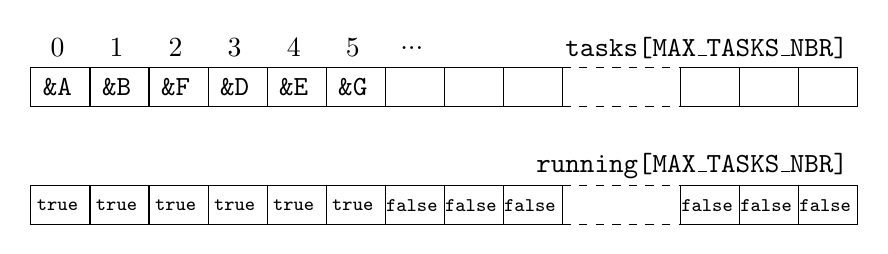
\begin{tikzpicture}[yscale=1, xscale=1.5]
        % \draw[help lines] (-5,-1) grid (5, 2);

        \draw node at (-4.775, 1.25) {0};
        \draw node at (-4.275, 1.25) {1};
        \draw node at (-3.775, 1.25) {2};
        \draw node at (-3.275, 1.25) {3};
        \draw node at (-2.775, 1.25) {4};
        \draw node at (-2.275, 1.25) {5};
        \draw node at (-1.775, 1.25) {...};

        \draw node[anchor=east] at (2, 1.25) {\texttt{tasks[MAX\_TASKS\_NBR]}};
        \draw[step=0.5] (-5.0, 0.5) grid (-0.5, 1);
        \draw[step=0.5] (+0.5, 0.5) grid (+2.0, 1);
        \draw[dashed] (-0.5, 1.0) -- (+0.5, 1.0);
        \draw[dashed] (-0.5, 0.5) -- (+0.5, 0.5);

        \draw node at (-4.775, 0.75) {\texttt{\&A}};
        \draw node at (-4.275, 0.75) {\texttt{\&B}};
        \draw node at (-3.775, 0.75) {\texttt{\&F}};
        \draw node at (-3.275, 0.75) {\texttt{\&D}};
        \draw node at (-2.775, 0.75) {\texttt{\&E}};
        \draw node at (-2.275, 0.75) {\texttt{\&G}};
        
        \draw[step=0.5] (-5.0, -0.5) grid (-0.5, -1);
        \draw[step=0.5] (+0.5, -0.5) grid (+2.0, -1);
        \draw[dashed] (-0.5, -1.0) -- (+0.5, -1.0);
        \draw[dashed] (-0.5, -0.5) -- (+0.5, -0.5);
        \draw node[anchor=east] at (2, -0.25) {\texttt{running[MAX\_TASKS\_NBR]}};

        \draw node at (-4.775, -0.75) {\scriptsize\texttt{true}};
        \draw node at (-4.275, -0.75) {\scriptsize\texttt{true}};
        \draw node at (-3.775, -0.75) {\scriptsize\texttt{true}};
        \draw node at (-3.275, -0.75) {\scriptsize\texttt{true}};
        \draw node at (-2.775, -0.75) {\scriptsize\texttt{true}};
        \draw node at (-2.275, -0.75) {\scriptsize\texttt{true}};
        \draw node at (-1.775, -0.75) {\scriptsize\texttt{false}};
        \draw node at (-1.275, -0.75) {\scriptsize\texttt{false}};
        \draw node at (-0.775, -0.75) {\scriptsize\texttt{false}};
        \draw node at ( 0.725, -0.75) {\scriptsize\texttt{false}};
        \draw node at ( 1.225, -0.75) {\scriptsize\texttt{false}};
        \draw node at ( 1.725, -0.75) {\scriptsize\texttt{false}};

    \end{tikzpicture}
    \caption{Schéma des tableaux tasks et running de l'ordonanceur (3)}
    \label{fig:async_scheduler_2}
\end{figure}